\chapter{Contributions}\label{chap:contributions}

\begin{sectionIntro}
    All the work I have done during this internship is related
    to the \gls{pfw}, which was briefly presented in section \ref{sec:parameter-framework}.
\end{sectionIntro}

% {{{1
\section{Parameter-framework mechanisms}
Should i really add this?

% {{{1
\section{Parameter-framework core enhancements}

% {{{2
\subsection{Improving build process}
\subsubsection{Build process}
The pfw language as described in \ref{desc:pfw-language} is used for rule based
description. Those are translated into \gls{xml} files during the build via a
specific make target.  In order to generate those \gls{xml} files, we also need
the information of the Structure files, which are written by the integration
engineers.

To generate those files, we rely on a toolset we call \emph{XmlGenerator}.
The figure \ref{fig:build-process} shows how it works:

\begin{figureGraphics}{Xml generation build process}{fig:build-process}
    \includegraphics[height=0.4\textheight]{./src/img/build-generation.pdf}
\end{figureGraphics}

But there were some limitations. Since the writing of the \gls{xml} structure files is done by human beings, there was
\emph{no guarantee} that their files were semantically correct.
Since no check was done during the build-process, the generator could write erroneous files because it supposes that
the Structure files are \emph{correct}. An example can be that someone forgot to specify the \emph{size} property of a parameter.
This lead to \emph{run-time errors} and \emph{undefined behaviour} because we are basically allocating zero memory for that parameter.

\subsubsection{Schemas}
To avoid strange run-time errors to bad generated files, we must make it impossible to generate erroneous files.
In order to do that we use \gls{xsd} files, which are describing what the content of an .xml element \emph{should be}.

Listing \ref{lst:xsd} shows a snippet example of an \gls{xsd} file:

\begin{lstlisting}[language=XML, caption=XSD rules for an Integer parameter, label=lst:xsd]
<xs:attributeGroup name="IntegerParameterAttributes">
    <xs:attribute name="Size" type="SizeType" use="required"/>
    <xs:attribute name="Min" type="xs:integer" use="optional"/>
    <xs:attribute name="Max" type="xs:integer" use="optional"/>
    <xs:attribute name="Signed" type="xs:boolean" use="optional" default="false"/>
</xs:attributeGroup>
\end{lstlisting}

In this code, we see that the \gls{xsd} is \emph{requiring} that we specify the \emph{Size} attribute.

\subsubsection{Xml checker}
We decided to integrate an automatic \gls{xsd} check at build time. In order to do so, I started writing a \gls{python} script
to integrate with the XmlGenerator tool. Since we wanted a more robust solution, It was finally done within the \gls{pfw} itself.

Figure \ref{fig:build-process-reworked} shows the final implementation and where we check the structure validity.

\begin{figureGraphics}{Xml generation build process with XSD check}{fig:build-process-reworked}
    \includegraphics[height=0.5\textheight]{./src/img/build-generation-after.pdf}
\end{figureGraphics}


% {{{2
\subsection{Multi-variant initial support}
TODO

\subsubsection{Alsa}
\subsubsection{Parameter-framework}


% {{{2
\subsection{Fixed point parameter enhancements}
The \gls{pfw} has several kinds of parameters:
\begin{itemize}
    \item IntegerParameter
    \item BooleanParameter
    \item FixedPointParameter
    \item StringParameter
    \item EnumParameter
    \item ...
\end{itemize}

Fixed point numbers are useful for representing fractional numbers. Their
usage is appropriate when the processor does not haves a floating point unit
or when there is a performance gain by using them. Usually, fixed points are
represented by $Qn.m$ format, where $n$ is the \emph{Integral part} and $m$ the
\emph{Fractional part}.

The implementation of fixed point numbers in the \gls{pfw} had some
corner cases which were not correctly handled. Round issues appeared when we
were writing to a configuration file or displaying user input. To
support the expected behavior for those cases, I changed the implementation, and
wrote tests for it.

\subsubsection{Test suite in Python}

In order to verify that the new implementation was correct, I wrote a test suite
in \gls{python}. That test suite performs several checks on each fixed point. Let's
take an example to illustrate the purpose of the test suite.

Let's take the case of a $Q2.3$ number: the \emph{Integral part} is $2$ and the
\emph{Fractional part} is $3$. We can compute some specific values for that number:

\begin{description}
    \item[Quantum] $2^{-3} = 0.125$
    \item[UpperBound] $2^2 - 0.125 = 3.875$
    \item[LowerBound] $-2^2 = -4$
\end{description}

Those values can be represented as following on figure \ref{fig:fixedPointValues}. Note that
this figure is not represented in real scale.
\begin{figureGraphics}{Fixed point special values}{fig:fixedPointValues}
    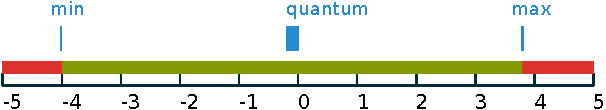
\includegraphics[width=\textwidth]{./src/img/fixedPoint.pdf}
\end{figureGraphics}


The test suite computes some values within the green(valid) area and the
red(invalid) area and performs the following checks on them:
\begin{description}
    \item[Bound check] The \gls{pfw} should throw an error if we
        attempt to set an out-of-bound value.
    \item[Sanity check] If we manage to set the value, The \gls{pfw} should not modify too much
        the value. It can only change by a quantum.
    \item[Consistency check] The \gls{pfw} should accept the value he sent us previously.
    \item[Bijectivity check] The \gls{pfw} should return us the same value we provided him at the Consistency check.
\end{description}

For a given value, the following test (view figure \ref{fig:fixedPointTest}) scenario is launched:
\begin{figureGraphics}{Fixed point test suite}{fig:fixedPointTest}
    \includegraphics[height=0.6\textheight]{./src/img/fixedPointProcess.pdf}
\end{figureGraphics}

\subsubsection{Rework the internal mechanism}
After that the test suite was implemented, it was time to rework the internal
mechanism of the \gls{pfw}.

The \gls{pfw} can export parameters towards a file. Fixed
point parameters can be exported as well.
\begin{itemize}
    \item When exporting them, the \gls{pfw} converts the value from
        its internal representation towards a floating point number, because that is
        easier to read.
    \item By converting that number, it also computes the amount of digits
        to use for display, or writing towards a file. This can result in
        \emph{rounding issues}, due to limitation of the \gls{cpp} method.
\end{itemize}
The fix I proposed was to replace the computation of displayable digits by something
easier, which is the \emph{Fractional part} of the fixed point number.

The example in listing \ref {lst:fixedPointProblem} illustrates a bound error error, and the output in the corrected version.
\begin{lstlisting}[caption=$Q.2.3$ rounding issue example, label=lst:fixedPointProblem]
####################
#  broken version  #
####################
$ pfw setParameter /Example/fixedPoint/q2.3 3.875
# Done
$ pfw getParameter /Example/fixedPoint/q2.3
# 3.9 <= this is not expected!
$ pfw setParameter /Example/fixedPoint/q2.3 3.9
# Value 3.9 standing out of admitted real range
# [-4, 3.875] for FixedPointParameter /Test/test/q2.3
# ^ this is even weirder

###################
#  fixed version  #
###################
$ pfw setParameter /Example/fixedPoint/q2.3 3.875
# Done
$ pfw getParameter /Example/fixedPoint/q2.3
# 3.875
\end{lstlisting}


% {{{2
\subsection{Multiple modem support}
With the bring your own device trends more and more smartphones support dual simcards. This implies that the platform must support two modems.
Within the Intel Audio \gls{hal}, we are

\subsubsection{Parameter-framework plugin}

% {{{1
\section{Open-sourcing on GitHub}
In order to stimulate the usage of the \gls{pfw} for other projects than the Intel Audio \gls{hal},
our team decided to release the source-code on GitHub.
This should favor external contributions via \gls{pullrequests} and motivate
the community to use the \gls{pfw}.

Around this activity, I covered several topics:
\begin{description}
    \item[Communicating, Documentating] the \gls{pfw} components.
    \item[Push, clean, enchance] the code to make it sure no proprietary
        elements are made public.
\end{description}

% {{{2
\subsection{Parameter-framework introduction}
\subsubsection{Discovery tutorials}\label{sec:tutorials}

At the start of my internship, I had to check out the \gls{pfw}'s
source code without any documentation. The idea was to have a fresh look at
this piece of software to determine if it was open-source ready, straightforward
to use, for someone who is unfamiliar with it.

While doing that, I struggled a bit with the basic usage of the framework. The
team decided that it would be nice to have some newcomer tutorials and examples,
for an easier adoption of the open-source community. So I wrote several
tutorials:
\begin{description}
    \item[Compile and install]
        is a step-by-step guide about how to get the \gls{pfw}'s sources,
        build it and install it as a standalone on Ubuntu.
    \item[Run a simple example]
        is a howto about running the \gls{pfw} command-line interface,
        such as \lstinline{remote-process} and \lstinline {test-platform}.  In
        this howto, the configuration and setting files are provided so that
        the user can focus on the results. The example covers music play-list
        changing based on a user's mood.
    \item[An introduction to the .pfw language]\label{desc:pfw-language}
        is a tutorial about the .pfw language. This language was
        created to simplify the writing of settings files for the
        \gls{pfw}. Those files are then converted into \gls{xml}, which is
        the only language the \gls{pfw} understands.
\end{description}
These tutorials have been written in \gls{markdown}, the standard format used
on GitHub.

% {{{2
\subsection{Parameter-framework's intellectual property}
Intellectual property is very important at Intel. The \gls{pfw} is released in
BSD license. All the source files must contain the correct BSD license header according
to Intel's open-source policy.

\subsubsection{license checker}
Since there are 279 source files released currently on GitHub, it seems a lot of
work to check all those files manually.
I wrote an internal tool \gls{python} which performs the license check semi-automatically.
The script usage is quite straightforward and showed in listing \ref{code:license}.

\begin{lstlisting}[language=bash, caption=License checker usage, label=code:license]
usage: license_updater.py [-h] [--cpp | --mk] license root_location

Scans recursively trough directories to find source code which should be
updated with a new license header.

positional arguments:
    license        the license type: ['gpl', 'bsd', 'private']
    root_location  the directory to start scanning

optional arguments:
    -h, --help     show this help message and exit
    --cpp          (default) scan for C++ files: ('h', 'c', 'hpp', 'cpp')
    --mk           scan for Android make files: .mk
\end{lstlisting}


% {{{2
\subsection{Branch sync process}
Since we work internally on the \gls{pfw} and can receive external contributions via \gls{pullrequests},
it is quite difficult to keep the two repositories in sync.
On figure \ref{fig:branch-process} we can see how we manage to synchronize the different code.

\begin{figureGraphics}{Final branch process}{fig:branch-process}
    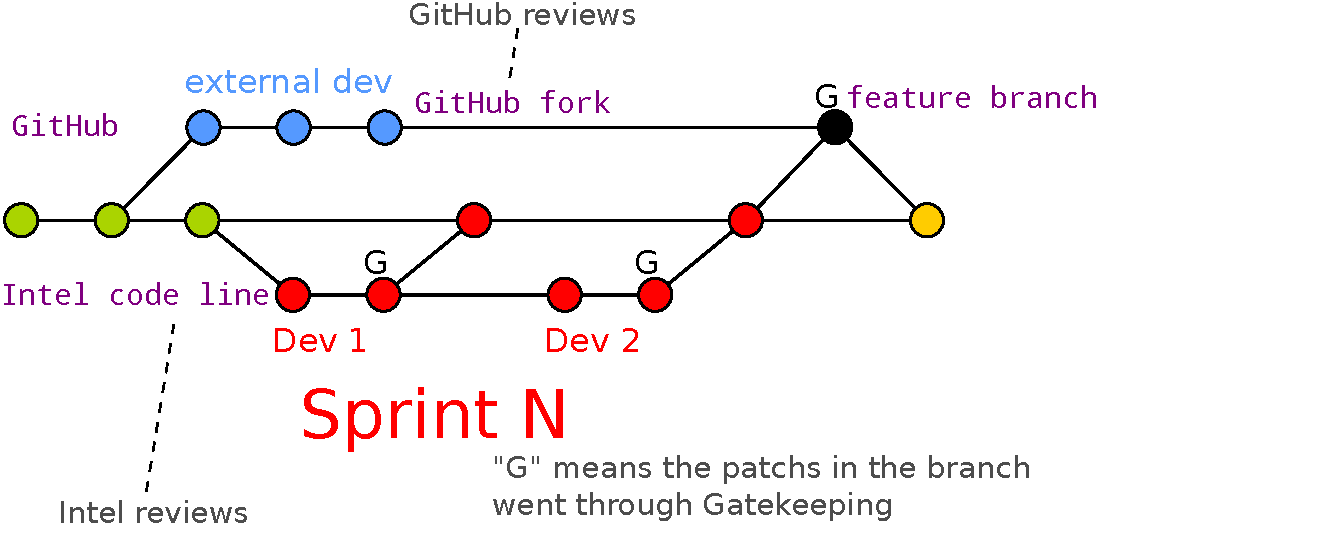
\includegraphics[width=\textwidth]{./src/img/branches-process.pdf}
\end{figureGraphics}


% {{{2
\subsection{Alsa plugin refactoring}
The Alsa plugin is used to handle Alsa or TinyAlsa subsystems.
For our internal uses, we have patched some \gls{aosp} projects.
This allows us to support different controls.
That control support was also visible in the Alsa \gls{pfw} plugin. Since
we want to open-source the plugin, those proprietary features should be removed.

During the removal of those proprietary features, we also simplified the plugin
architecture by merging the controls and the mixer code.
This results in a far simpler design.

% {{{2
\subsection{Core upload}
Open-sourcing the \gls{pfw} required some initial work.
In order to smoothly integrate features from external contributors and internal work,
Requirements, vanilla \gls{aosp}, internal tree and open-source version must be the
same.
01org organisation, Intel open-source technology center.

The project is available at \url{https://github.com/01org/parameter-framework}

% {{{2
\subsection{File system plugin upload}

The project is available at \url{https://github.com/01org/parameter-framework-plugins-filesystem/}

% {{{2
\subsection{Alsa plugin upload}
\subsubsection{Alsa}
\subsubsection{Tinyalsa}
\subsubsection{Plugin architecture}
CTL and MIX merged

The project is available at \url{https://github.com/01org/parameter-framework-plugins-alsa/}
